\documentclass[12pt]{article}
\title{%
The Effects of Phenotypic Plasticity on the Fixation Probability of Mutant Cancer Stem Cells}
\author{Brydon Eastman}
\usepackage[margin=3cm]{geometry}
\usepackage{amsmath,amsfonts,amsthm,amssymb,graphicx,float}

\graphicspath{{../images/}}

\usepackage[title]{appendix}

\usepackage{microtype, url}
\renewcommand{\d}{{\rm d}}
\begin{document}
\maketitle
\begin{abstract}
The cancer stem cell hypothesis claims that tumor invasion, metastasis, and maintenance is driven by a small niche of the total cancer cell population called Cancer Stem Cells. These CSCs can differentiate into specialised, progenitor cells or reproduce into new CSCs. While it was once held that this differentiation pathway was unidirectional, recent research has demonstrated that differentiated cells are more plastic than initially considered. In particular, differentiated cells can de-differentiate and recover their stem-like capacity. Two recent papers have considered how this rate of plasticity affects the evolutionary dynamic of an invasive, malignant population of stem cells and differentiated cells into existing tissue \cite{mohammad, wodarz}. These papers arrive at seemingly opposing conclusions, one claiming that increased plasticity results in increased invasive potential, and the other that increased plasticity decreases invasive potential. This report demonstrates that what really matters when determining the effect on invasive potential is how one distributes this increased plasticity between the compartments of resident and mutant-type cells.
\end{abstract}
\section{Introduction}
Cancer invasion is a complex process of the cellular ecosystem and micro-environment. Typically, cancerous cells achieve evolutionary success by mimicking, and subverting, the behaviour of regular, healthy tissues in the host \cite{moh1}. In healthy tissue a distinct stratification of tissue structure is observed where the self-renewal capabilities of terminally differentiated cells rely upon a discrete subclass of the cellular population deemed stem cells \cite{weis2000}. In particular, these stem cells can behave invasively through the process of division and specialisation \cite{moh2}. As healthy, specialised (or differentiated) cells die, the stem cells divide producing the required differentiated cell as a byproduct of mitosis. In this way the population of specialised, terminally differentiated cells is maintained \cite{moh2, watt2000}. However, in order to maintain tissue homeostasis, this mechanism must be controlled by both positive and negative feedback loops. To that effect there is mounting evidence that differentiated cells can de-differentiate back into adult stem cells \cite{watt2000}.

This process of cellular invasion in the tissue driven by a particular niche of cells is very similar to the dynamics observed in invasive cancers. This has led to the cancer stem cell hypothesis that posits that the invasion, metastasis, and regulation of solid tumors are driven by a small sub-population of cells that behave very much like stem cells \cite{moh3, moh4, moh5, moh6}. In particular, this same behaviour of differentiated cells undergoing some process of de-differentiation and recovering some stem-like properties has been implicated in many forms of cancers experimentally \cite{moh23, moh24, moh25, moh26}.

Recently two papers have mathematically modeled the effect of this stem-cell plasticity and de-differentiation on the evolutionary dynamics of cancer stem cells \cite{mohammad,wodarz}. Both papers are concerned with how the invasive efficacy of mutated stem cells depends upon the degree of de-differentiation considered. In particular, both investigate a situation where a resident type of stem cells and differentiated cells have fully saturated within a population and by introducing a single mutant type within the population the fixation probability of these mutants is recovered. In \cite{mohammad} the authors conclude that as the rate of plasticity increases in a population of cancer stem cells, the fixation probability of mutant stem cells increases. In \cite{wodarz}, however, the authors conclude that as the plasticity increases in a population of cancer stem cells, the fixation probability of mutant stem cells decreases. These results are evidently at odds with one another and it is the purpose of this report to reconcile and explain the differing dynamical predictions of these models.
\section{Modeling}

The situation being modeled is the same in both papers \cite{mohammad, wodarz}. The authors consider a population of resident stem cells in an equilibrium state. They then introduce a mutant, cancerous stem cell into the wild-type population and investigate the probability that the single mutant achieves fixation as a function of the plasticity of the mutant stem cell. That is, the probability $\rho_S$ that as time $t$ tends to infinity the wild type stem cells have all either died or differentiated and the mutant type stem cells remain for a given de-differentiation rate $\eta$.

\subsection{A Discrete Moran Model}

In \cite{mohammad} the authors consider modeling the birth-death process by way of a Moran model. In particular, the authors consider two types of cells, stem cells ($S_i$) and differentiated cells ($D_i$) where $i\in\{1,2\}$ denotes whether the cells in question are wild-type ($i=1$) or mutant-type ($i=2$). Cells can react and transition between compartments according the following rules (summarised in Figure \ref{MohFig1}). Stem cells undergo mitosis at a rate $r_i$. There is a probability $u_i$ that the stem cell produces both a stem cell $S_i$ and a differentiated cell $D_i$ during division. Similarly, with probability $(1-u_i)$, the stem cell produces two stem cells as the result of this division. Moreover, differentiated cells can reproduce as well at a rate $\tilde{r}_i$. There is a probability $\eta_i$ that this division is asymmetric, producing one stem cell $S_i$ and one differentiated cell $D_i$, and a probability ($1-\eta_i$), that the division is symmetric, producing two differentiated cells $D_i$. Similarly, with probability $d_i$ and $\tilde{d}_i$, the stem cells and differentiate cells die.

\begin{figure}[!ht]
\begin{center}
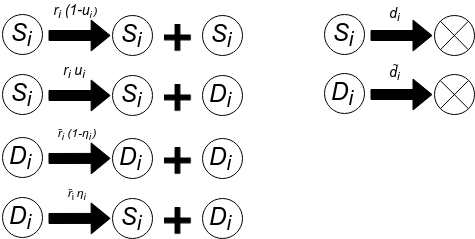
\includegraphics[width=0.9\textwidth]{moh_rxn.png}
\end{center}
\caption{The differentiation, de-differenation, and death events corresponding to a four-compartment model where $S_i$ and $D_i$ are the stem-cells and differentiated cells for the wild-type ($i=1$) and mutant-type ($i=2$) respectively. Differentiation and de-differentiation events connect the selection dynamics between the two niches.}\label{MohFig1}
\end{figure}


Note that in each of these events the population of stem cells and differentiated cells changes by at most 1 in either direction. Moreover, as births and deaths of cells are assumed to occur instantaneously, the state of the system at any point in time is determined entirely by the state at the previous time. Hence, the particular stochastic process being considered is Markovian. Further, the authors assume that each individual compartment has constant population size across wild and mutant types: i.e. the number of stem cells and the number of differentiated cells remain static, merely what proportion of these stem or differentiated cells are wild or mutant type is what changes. 

Let $N_S$ denote the size of the stem cell compartment, $N_D$ the size of the differentiated compartment, and $N=N_S+N_D$ the total number of cells considered. Further, we are concerned primarily with invasion of mutant types; that is, when the number of $S_2$ or $D_2$ cells is at a maximum (equal to $N_S$ or $N_D$). Hence we let $n_S$ and $n_D$ represent the number of $S_2$ or $D_2$ cells. Therefore, the number of $S_1$ or $D_1$ cells is given by $N_S-n_S$ and $N_D-n_D$, respectively. Let $W_S^+(n_S,n_D), W_S^-(n_S,n_D), W_D^+(n_S,n_D)$, and $W_D^-(n_S,n_D)$ represent the transition probabilities corresponding to an increase or decrease by one (represented by the $+$ or $-$ in the superscript) in the number of stem cells or differentiated cells (represented by the $S$ or the $D$ in the subscript) Then if $1/N$ is the duration of each time step in this model, one can represent the following master equation for the probability density function of the stochastic process as follows:

\begin{align}
\frac{1}{N}\frac{\partial p(n_S,n_D;t)}{\partial t}&=W_S^+(n_S-1,n_D)\, p(n_S-1,n_D;t) + W_S^-(n_S+1,n_D)\, p(n_S+1,n_D;t)\nonumber\\
&\quad
+ W_D^+(n_S,n_D-1)\, p(n_S,n_D-1;t) + W_D^-(n_S,n_D+1)\, p(n_S,n_D+1;t)\nonumber\\
&\quad
-(W_S^+(n_S,n_D)+W_D^+(n_S,n_D)+W_S^-(n_S,n_D)+W_D^-(n_S,n_D))\, p(n_S,n_D;t)
\label{MohRef1}
\end{align}

Where the transition probabilities are given as follows:
\begin{align}
W_S^+(n_S,n_D) &= \left(r_2\,(1-u_2)\,n_S+\tilde{r}_2\,\eta_2\,n_D\right)\left(\frac{N_S-n_S}{N_S}\right)\label{MohRef2}\\
W_S^-(n_S,n_D) &= \left(r_1\,(1-u_1)\,(N_S-n_S)+\tilde{r}_1\,\eta_1\,(N_D-n_D)\right)\left(\frac{n_S}{N_S}\right)\\
W_D^+(n_S,n_D) &= \left(\tilde{r}_2\,(1-\eta_2)\,n_D+r_2\,u_2\,n_S\right)\left(\frac{N_D-n_D}{N_D}\right)\\
W_D^-(n_S,n_D) &= \left(\tilde{r}_1\,(1-\eta_1)\,(N_D-n_D)+r_1\,u_1\,(N_S-n_S)\right)\left(\frac{n_D}{N_D}\right).
\label{MohRef3}
\end{align}

With equations (\ref{MohRef1}) and (\ref{MohRef2}-\ref{MohRef3}) are reproduced from \cite{mohammad}.

\begin{figure}[!ht]
\begin{center}
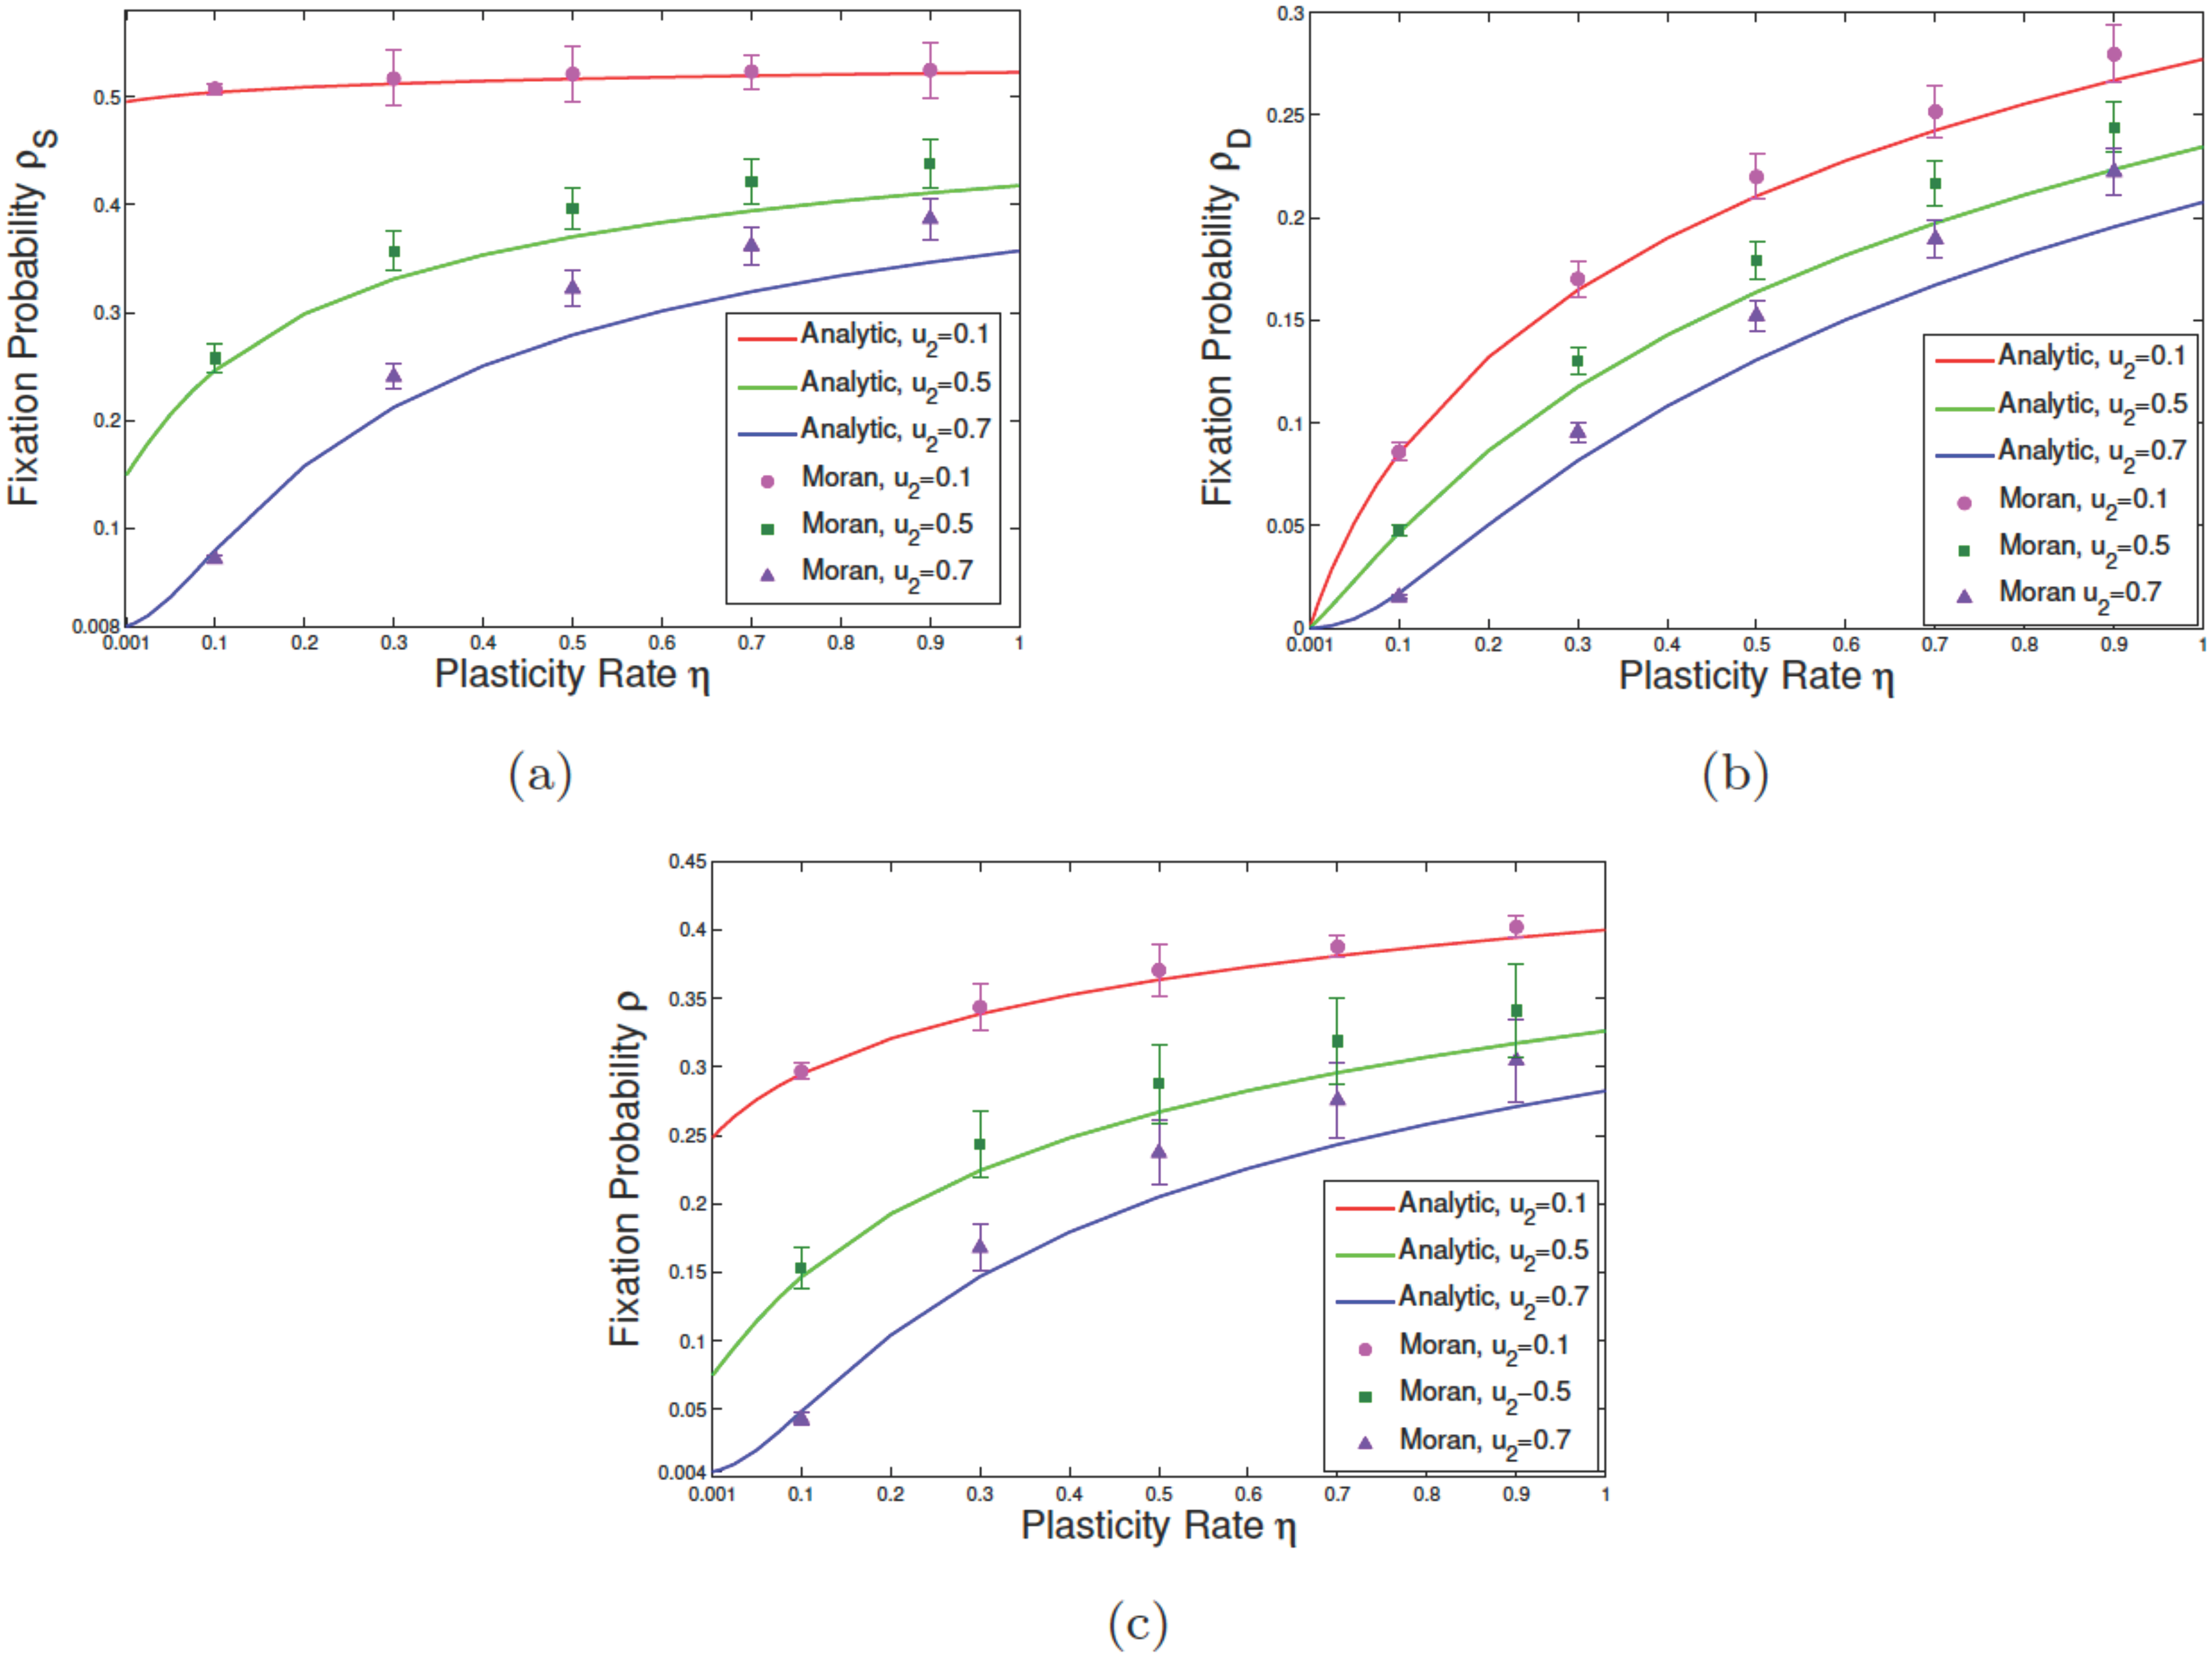
\includegraphics[width=0.9\textwidth]{moh_fig5.png}
\end{center}
\caption{Effect of Change in the rate of phenotypic plasticity for mutant DCs on the survival probability of malignant cells. In subfigures (a), (b), and (c) we have respectively considered the fixation probability of mutants while the initial malignant mutation respectively occurs in SC, DC, and SC+DC compartments at random. In these plots $N_S=N_D=10$, $r_1=\tilde{r}_1=1$, $r_2=\tilde{r}_2=1.1$, $u_1=0.5$, and $\eta_1=0$. Different asymmetric division rates of normal and malignant individuals have also been taken into account when the fixation probability is given as a function of $\eta$. Solid curves and points are respectively the results of exact calculations and simulation analyses. At each given discrete point, the error bar depicts the standard error of the mean. Reproduced from \cite{mohammad}.}\label{MohFig5}
\end{figure}

The results of Figure \ref{MohFig5} clearly demonstrate that fixation probability increases as plasticity of the mutant increases. In particular, when the resident wild type cells were given no plasticity and the mutant type cells plasticity was treated as a variable it was observed that increasing the mutant types plasticity gave these mutant types a greater invasive potential when placed in a population dominated by wild types population.


\subsection{A Continuous Gillespie Model}
On the other hand, in \cite{wodarz}, the author wishes to describe the dynamics of stem cell invasion not merely by considering births and deaths and the selective pressures therein, but by directly considering the positive and negative feedbacks that control differentiation and de-differentiation in the stem cell hierarchy. To this end, the author constructs multiple systems of differential equations that model the behaviour of stem cells and differentiated cells under various assumptions. The key differences between this paper and \cite{mohammad}, are in the details of these models. In particular, the author does not limit themselves to constant population size of stem cell and differentiated cell compartments. As before, the author considers a four compartment model where $S_i$ represents the stem cells and $D_i$ represents the differentiated cells. 

\begin{equation}
\begin{array}{rl}
\frac{\d S_i}{\d t}&= \hat{r}_i\,S_i\,(2\,p_i-1)+g_i\,D_i\vspace*{5pt}\\
\frac{\d D_i}{\d t}&= 2\,\hat{r}_i\,S_i\,(1-p_i)-\alpha_i\,D_i-g_i\,D_i
\end{array}
\end{equation}\label{wodDE}
where $i\in\{1,2\}$ represents the wild type ($i=1$) and mutant type ($i=2$), as before.

While the author of \cite{wodarz} does not frame the model as a reaction network, it is not hard to recover the set of reactions from the differential equations. These are presented in Figure \ref{wodarzRxns}. 

\begin{figure}
\begin{center}
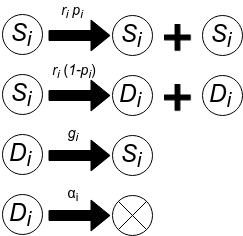
\includegraphics[width=0.4\textwidth]{wodarz-rxns.png}
\end{center}
\caption{Figure demonstrating the suite of reactions captured by the Wodarz Model. Stem cell division is always assumed to be symmetric, producing either two new stem cells or two progenitor cells.}\label{wodarzRxns}
\end{figure}

The author does not consider the differential equations exactly as written, it is not hard to see why. In particular, if $p_i\neq \frac{\alpha_i-g_i}{2\,\alpha_i}$, then the only equilibrium is $S_i=D_i=0$. Otherwise, the entire set $[S_i,D_i]=[S_i,(r_i/\alpha_i)\,S_i]$ is an equilibrium. 

These results do not coincide with what is observed in experiments. The author argues that feedback on the division rate, self-renewal probability, and de-differentiate rate occurs in order to maintain finite-size cell populations. To model this the author considers $\hat{r}_i$, $p_i$, and $g_i$ to be decreasing functions of the cell population sizes in the following way
\[
\hat{r}_i=\frac{\hat{r}_i'}{1+h_{i,1}\,D_i^{k_{i,1}}}, \quad p_i=\frac{p_i'}{1+h_{i,2}\,D_i^{k_{i,2}}}, \quad g_i=\frac{g_i'}{1+h_{i,3}\,S_i^{k_{i,3}}}
\]
In this case, the model permits an equilibrium point internal to the first quadrant that is stable when $p_i>\frac{\alpha_i-g_i}{2\,\alpha_i}$.

To numerically establish the fixation probability the following experiments were run. The author begun by placing $S_1$ and $D_1$ at the equilibrium values and then introduced a single mutant stem cell, $S_2=1$ and $D_2=0$. Gillespie simulations were then performed \cite{gillespie} for many realisations (more than $10^8$). The fraction of simulations in which the mutants fixated was recorded and from this the fixation probability was estimated. This was done for various values of de-differentiation rates $g=g_1=g_2$. The results are recorded in Figure \ref{wodarzResults}.

\begin{figure}[!ht]
\begin{center}
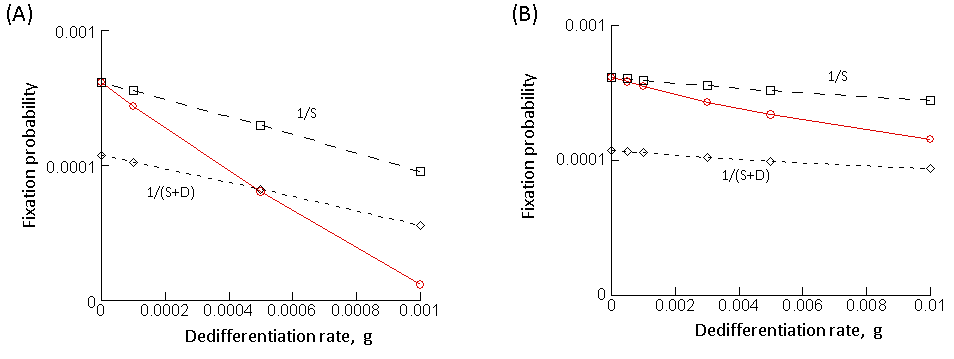
\includegraphics[width=0.9\textwidth]{wodarz.png}
\end{center}
\caption{Effect of de-differentiation on the fixation probability of a neutral mutant, determined by computer simulations. Gillespie simulations of the model were run. A single mutant was placed into a resident cell population at equilibirum, and the fraction of realisations that resulted in the fixation of the mutant was recorded. This was done for a case without de-differentiation ($g=0$) and for cases with varying rates of de-differentation. This is depicted by the red, solid line the plots. The black dashed lines indicate reference values, such as $1/S_1^\ast$, the inverse of the equilibrium number of resident stem cells, which according to evolutionary theory, should equal the fixation probability of a neutral mutant. Since the mutant is neutral, all $i$ subscripts are omitted from parameter values as they are the same (i.e. $p'_1=p'_2=p'$). (A) Model without feedback on de-differentiation; $\hat{r}'=0.01$; $p'=0.8$; $\alpha=0.0025$; $h_1=h_2=0.0001$; $k_1=k_2=1$; $h_3=0$, $k_3=1$. (B) model with feedback on de-differentiation; same parameters and $h_3=0.01$, $k_3=1$. Reproduced from \cite{wodarz}.}\label{wodarzResults}
\end{figure}

In contrast to the results of \cite{mohammad}, Figure \ref{wodarzResults} shows that the fixation probability of a neutral mutant decreases when the de-differentiation rate increases.

\section{Reconciliation of Previous Results}\label{recon}

In the Wodarz model there are four parameters considered for each cell-type (mutant or wild) ($p_i, \hat{r}_i, \alpha_i, g_i$) while in the Shirayeh model there are six ($r_i,\tilde{r}_i, d_i, \tilde{d}_i, \eta_i, u_i$). The biggest difference between these parameters is that in the Wodarz model the numbers $p_i$ and $r_i$ are both functions of $D_i$ and $g_i$ is a function of $S_i$.

Moreover, the Wodarz model considers four reactions between stem cell and differentiated cell compartments \[S_i\to S_i+S_i, S_i\to D_i+D_i, D_i\to S_i, D_i\to \emptyset.\] Whereas in the Shirayeh model there are six
\[
S_i\to S_i+S_i, S_i\to S_i+D_i, D_i\to D_i+D_i, D_i\to D_i+S_i, S_i\to\emptyset, D_i\to\emptyset.
\]

However, all the reactions from the Shirayeh model can be recovered in the Wodarz model. In particular, in order for stem cells to die they must first differentiate and then the differentiated cells must both die. In order to obtain asymmetric stem cell division, the stem cells must first divide into two differentiated cells, then one of the differentiated cell must de-differentiate back into a stem cell. Suppose a differentiated cell first differentiates into a stem cell and then the resultant stem cell symmetrically differentiates. Therefore, the differentiated cell has symmetrically divided. Further, suppose one of those resultant differentiated cells de-differentiates back into a stem cell, then the differentiated cell has asymmetrically divided. In this way all the reaction dynamics of the model from \cite{mohammad} have been recovered by multiple reactions from the model by \cite{wodarz}.

This realisation lends credence to the theory that the models should, hopefully, predict similar qualitative dynamics. To that end, we begin by creating differential equations via the reactions given in Figure \ref{MohFig1} and compare them to the differential equations presented in \cite{wodarz}. By making the mass-action assumption, it is easy to derive
\begin{equation}
\begin{array}{rl}
\frac{\d S_i}{\d t}&=\tilde{r}_i\,\eta_i\,D_i+r_i\,(1-u_i)\,S_i-d_i\,S_i\vspace*{5pt}\\
\frac{\d D_i}{\d t}&=\tilde{r}_i\,(1-\eta_i)\,D_i+r_i\,u_i\,S_i-\tilde{d}_i\,D_i.
\end{array}
\end{equation}\label{mohDE}
Contrasting (\ref{mohDE}) with (\ref{wodDE}) it is not hard to derive the following relations.

To frame the Wodarz model in terms of parameters from the Shirayeh model,
\begin{align*}
p_i&=1-\frac{r_i\,u_i}{2\,(r_i-d_i)}\\
\hat{r}_i&=r_i-d_i\\
\alpha_i&=\tilde{d}_i-\tilde{r}_i\\
g_i&=\tilde{r}_i\,\eta_i
\end{align*}
conversely, framing the Shirayeh model in terms of parameters from the Wodarz model we leave $d_i$ and $\tilde{d}_i$ as free parameters, then
\begin{align*}
r_i&=d_i+\hat{r}_i\\
\tilde{r}_i&=\tilde{d}_i-\alpha_i\\
\eta_i&=\frac{g_i}{\tilde{d}_i-\alpha_i}\\
u_i&=2\frac{\hat{r}_i\,(1-p_i)}{d_i+\hat{r}_i}.
\end{align*}

Hence the qualitative dynamics of Model \ref{mohDE} are dynamically equivalent to those of Model \ref{wodDE}, under a renaming of parameters. Moreover, these formulae allow us to more carefully compare the two systems predictions under differing notations and parameter choices, as the formulae provide a way to transcribe parameter values and notational choices from one system into the notation of the other. In particular, note that the two plasticity parameters $g_i$ and $\eta_i$ can be compared directly, as they are just linear, increasing functions of one another. Hence an increase in $g_i$ is analogous to an increase in $\eta_i$ (and vice versa). Moreover, $\eta_i=0$ is analogous to $g_i=0$.

Negative feedback on production rates is modeled in the model put forth by \cite{mohammad}, but not as explicitly as in \cite{wodarz}. In particular, the last factor in the transition probabilities of \cite{mohammad} provide this bias. If $n_S$ is high, or the number of stem cells is close to maximum, then the transition probability $W_S^+$ is near zero, due to the $(N_S-n_S)/N_S$ factor at the end. Hence when the number of mutant stem cells is high, the probability of making more mutant stem cells is lowered (this mimics the behaviour observed in the $g_2(S_2)$ function in the Wodarz model). Similarly the $n_S/N_S$ term in the $W_S^-$ transition probability creates pressure where creating more wild-type stem cells is less likely in the presence of many wild-type stem cells (similar to the $g_1(S_1)$ function in the Wodarz model). Analogous behaviour occurs in the $W_D^{\pm}$ probabilities, mimicking the behaviour of the $\hat{r}_i$ and $p_i$ functions decreasing as $D_i$ increases. 

In the finite population size model, negative feedback on (de-)differentiation rates and production rates are governed by the select pressures inherit in finite population sizes, whereas in the unbounded population size model these same feedback mechanisms are modeled by non-constant, non-linear reaction rates. 

A more subtle difference between the two systems is due, in part, to a lack of clarity in notational differences. In the original presentation of \cite{wodarz} the $i$ subscripts were not present (though different values of the same parameter between compartments was implied in the figure descriptions). Among other things, this obscures the fact that $g$ (the parameter representing de-differentiation, or plasticity) is being altered at the same rate for both the mutant-type population and for the resident-type population. Hence, the plots in Figure \ref{wodarzResults} really plot the fixation probability $\rho_S(g_1,g_2)$ along the diagonal cross-section of the first quadrant, that is the plots show
\[
\frac{\partial}{\partial g}\left(\rho_S(g_1,g_2)\big|_{g_1=g_2=g}\right)<0
\]
whereas the plots in Figure \ref{MohFig5} show
\[
\frac{\partial}{\partial \eta_2}\left(\rho_S(\eta_1,\eta_2)\big|_{\eta_1=0}\right)>0.
\]
The tacit assumption in \cite{mohammad} is that part of the phenotypic difference between the mutant stem cells and the resident stem cells is that resident stem cells have no plasticity and mutant stem cells do have plasticity. The analysis then focuses around qualifying the effects of this plasticity. Contrast this, the tacit assumption in \cite{wodarz} is that the mutant and resident stem cells are phenotypically different in some other way and share the same plasticity rate.


\subsection{Recreating the Dynamics from the Gillespie Model in the Moran Model}
To investigate this further, we first considered the Moran process as before (from \cite{mohammad}), except measuring $\rho_S(\eta, \eta)$ for various values of $\eta$. The results can be seen in Figure \ref{mohBothInc}. In particular, note that $\rho_S(0,\eta)$ is an increasing function of $\eta$, as was previously observed in \cite{mohammad} (and Figure \ref{MohFig5}). However, $\rho_S(\eta, \eta)$ is a \textit{decreasing} function of $\eta$, analogous to what was observed in \cite{wodarz} (and Figure \ref{wodarzResults}).


\begin{figure}[!ht]
\begin{center}
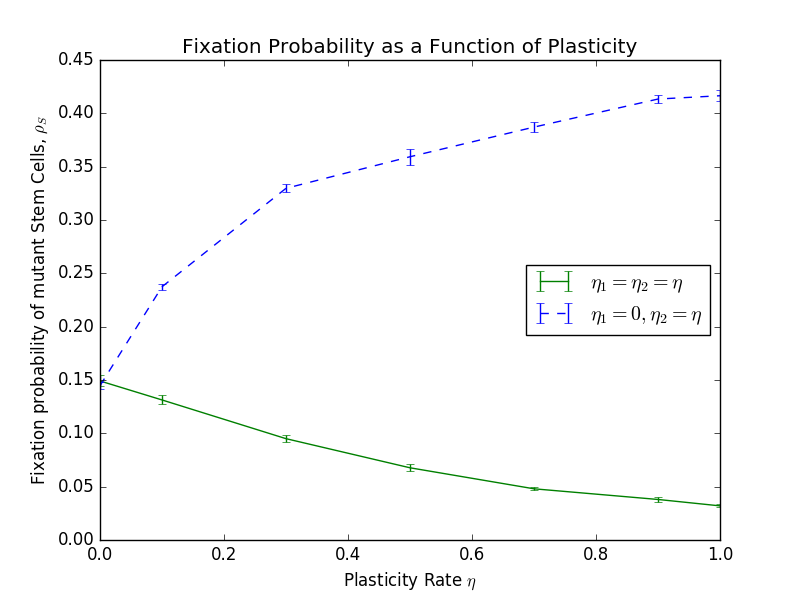
\includegraphics[width=0.7\textwidth]{moh_both.png}
\end{center}
\caption{A plot conceptially similar to the green (middle) line in Figure \ref{MohFig5} (a). This plot shows the Moran model from \cite{mohammad} with $r_2=\tilde{r}_2=1.1$, $u_1=u_2=0.5$, $r_1=\tilde{r}_1=1$, and $\eta$ taking values in $\{0, 0.1, 0.3, 0.5, 0.7, 0.9, 1\}$. The dashed, blue line indicates $(\eta_1, \eta_2)=(0,\eta)$ (effectively recreating the middle line in Figure \ref{MohFig5} (a)) and the solid, green line indicates $(\eta_1, \eta_2)=(\eta, \eta)$. The error bars are standard error of the mean. Each point is the mean of five simulations run. Each simulation runs the Moran model 2,000 times for 15,000 time steps. }\label{mohBothInc}
\end{figure}

\subsection{Recreating the Dynamics from Moran Model in the Gillespie Model}
Similarly, we considered the Gillespie process as from \cite{gillespie}. We have modeled both $\rho_S(0, g)$ and $\rho_S(g, g)$. Again, recognise that $\rho_S(0, g)$ is an increasing function of $g$ while $\rho_S(g, g)$ is a decreasing function of $g$, analogous to the results in Figure \ref{mohBothInc}.

\begin{figure}[!ht]
\begin{center}
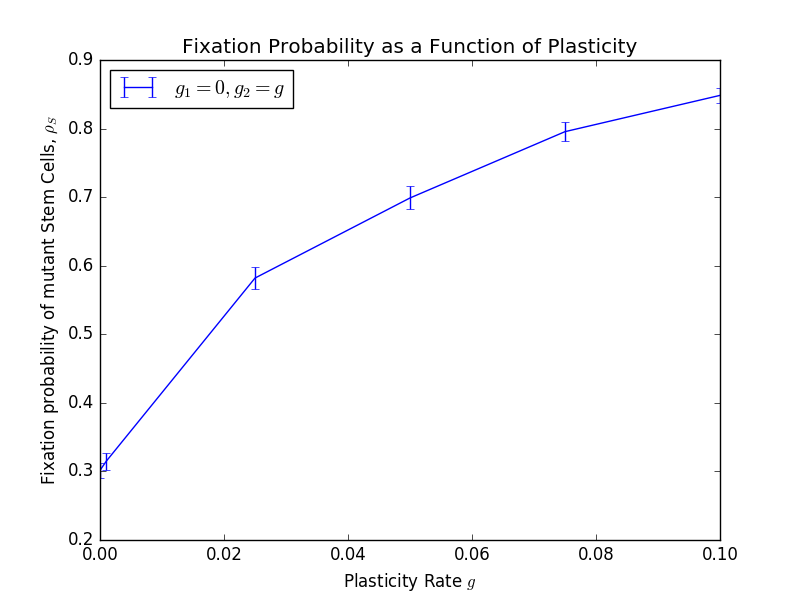
\includegraphics[width=0.74\textwidth]{gill_fix.png}
\end{center}
\caption{The fixation probability of a Gillespie model from \cite{wodarz} with feedback on division rate, renewal rate, and differentiability. However, the plasticity parameters $g_i$ were treated as distinct, with differing values. Contrast the qualitative shape with that of Figure \ref{wodarzResults} (B) that models the same stochastic process. Here $\hat{r}'=1, p'=0.6, \alpha=0.105, h_1=h_2=h_3=0.01, k_1=k_2=k_3=1,$ and finally $g_1=0, g_2=g$ for $g\in\{0,0.001,0.025,0.050,0.075,0.100\}$.}\label{GillFix}
\end{figure}

\section{Further Results}
The results of Section \ref{recon} demonstrate that it is vitally important to consider how a change in plasticity in a mutant type affects a change in plasticity of a wild type, if at all.
In particular, the authors of \cite{mohammad} and \cite{wodarz} were effectively answering different research questions. In \cite{mohammad} the authors were concerned with what the effect of increased plasticity in a mutant-type would have on fixation probability assuming the wild-type stayed the same. This corresponds to a case where the mutant-type gains increased plasticity as part of the mutation. Moreover, this assumes that this increased plasticity in the mutant type does not have any effects on the plasticity in the resident type. Contrarily, in \cite{wodarz} the authors assume that the increased plasticity is common to both the mutant and wild type stem cells. This could be the case where an increased mutant-type plasticity affects the wild-type stem cells by some kind of increased selective pressure, or via a change in the micro-environment thus influencing the wild-type to also become more plastic.

As Section \ref{recon} made it apparent that the Gillespie model and Moran model are effectively equivalent means of modeling this phenomenon, we consider Moran simulations henceforth. This is done purely because Moran simulations are less computationally expensive than Gillespie simulations.

We consider varying both $\eta_1$ and $\eta_2$ (the plasticity of the wild-type and mutant-type cells) independently of one another. Since $\eta_1$ and $\eta_2$ are probabilities, we varied them over the closed unit square $[0,1]\times[0,1]$ in a $36\times36$ grid. At each point in the grid we calculated the fixation probability of the mutant-type stem cells. Further details of the numerical simulation, and a link to the code, can be found in Appendix \ref{exp}. 

The purpose of the experiment was to further investigate the exact interplay between plasticity in the two compartments on the fixation probability. However, there are 6 other parameters to consider,  $r_i, \tilde{r}_i,$ and $u_i$. In order to investigate the direct effect of a change in plasticity on the fixation probability in isolation, we considered the case where relative fitness was the same in the stem and differentiated cells (that is, $r_i=\tilde{r}_i$).

We further considered experiments where the relative fitness of the mutant-type cells ($r_2=\tilde{r}_2$) were varied along with the de-differentiation probabilities ($\eta_1$ and $\eta_2$). Moreover, to further analyse the stability, we considered varying the differentiation probability ($u_2$) of the mutant-type cells along with the de-differentiation probabilities.

In the case of the neutral mutant (where $r_2=\tilde{r}_2=r_1=\tilde{r}_1$ and $u_2=u_1$), the results are summarised in Figures \ref{contour}, \ref{constantEta1Stack}, \ref{avg_eta1_plot}. The contour plot in Figure \ref{contour} indicates the fixation probability as a function of both de-differentiation parameters. It indicates that in general, increasing $\eta_2$, the de-differentiation probability of the mutant cells, increases the fixation probability. Moreover, this fixation probability is maximal for $(\eta_1, \eta_2) = (0, 1)$. However, it also shows that for large enough $\eta_1$, increasing $\eta_2$ will not always result in an increased fixation probability. In the extreme case, where $\eta_1=1$, increasing $\eta_2$ initially increases the fixation probability, but eventually this fixation probability decreases as $\eta_2$ is closer to $1$.

\begin{figure}[!ht]
\begin{center}
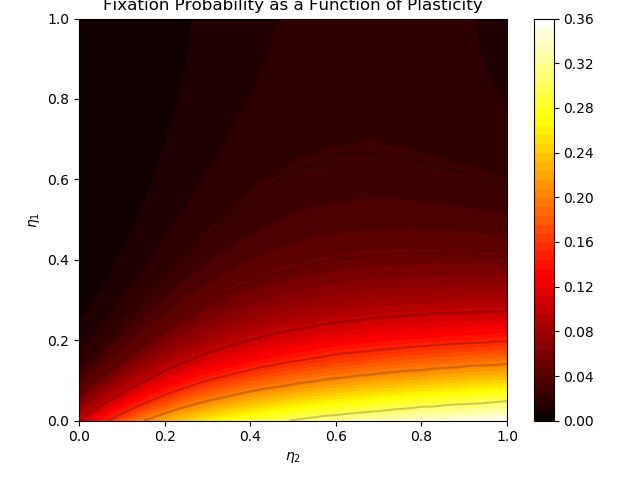
\includegraphics[width=0.74\textwidth]{contourplot.png}
\end{center}
\caption{A contourplot demonstrating the fixation probability as a function of both de-differentiation parameters. It indicates that increasing the mutant-type de-differentiation parameter does not always result in increased fixation of mutant-type stem cells, even when keeping the wild-type de-differentiation parameter constant.}\label{contour}
\end{figure}

This result can be seen more clearly in Figure \ref{constantEta1Stack}, where the fixation probability is plotted for constant values of $\eta_1$ as a function of varying $\eta_2$. When $\eta_1=0$ the fixation probability is a concave down, increasing, saturating function of $\eta_2$. However, for $\eta_1=0.2$ the fixation probability is still increasing, but undergoes a change in concavity early on. As $\eta_1$ is increased further the fixation probability is no longer a strictly increasing function of $\eta_2$ but initially increases and eventually decreases as $\eta_2$ becomes larger.

\begin{figure}[!ht]
\begin{center}
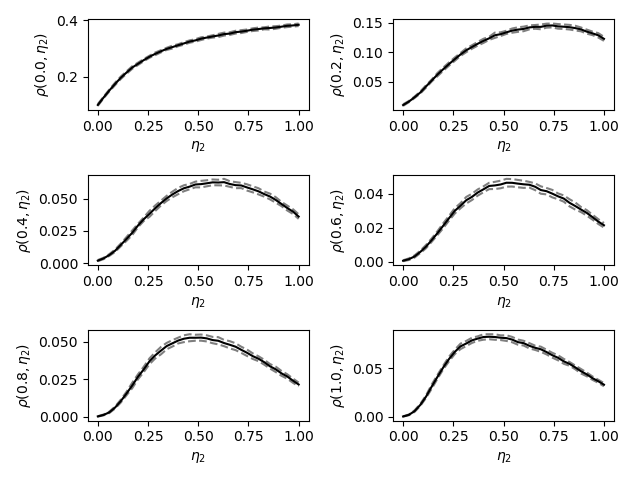
\includegraphics[width=0.74\textwidth]{constant_eta1_stackplot.png}
\end{center}
\caption{A stackplot demonstrating the fixation probability as a function of the de-differentiation probability $\eta_2$ for various choices of $\eta_1$. The solid line is the calculated fixation probability and the dashed lines indicate one deviation by the standard error of the mean.}\label{constantEta1Stack}
\end{figure}

When examining Figure \ref{contour}, it appears that in general the fixation probability increases. Moreover, when the fixation probability is increasing, it obtains a larger value. That is, for increasing $\eta_1$ the fixation probability is, in general, decreasing. This effect raises the question that in general, in a heterogeneous population of wild-type stem cells where deviations in de-differentiation probability $\eta_1$ can be observed, what might be the expected effect on the fixation probability. To that end, we modeled the average fixation probability as a function of $\eta_2$ averaged over all values of $\eta_1$. That is,

\[\langle\rho_S(\eta_2)\rangle = \int_0^1 \rho_S(\eta_1, \eta_2)\,f(\eta_1)\,\d \eta_1\]
where $f(\eta_1)$ is the probability density function for $\eta_1$ in this case taken to be uniform. The result, as presented in Figure \ref{avg_eta1_plot}, is an increasing function of $\eta_2$.

\begin{figure}[!ht]
\begin{center}
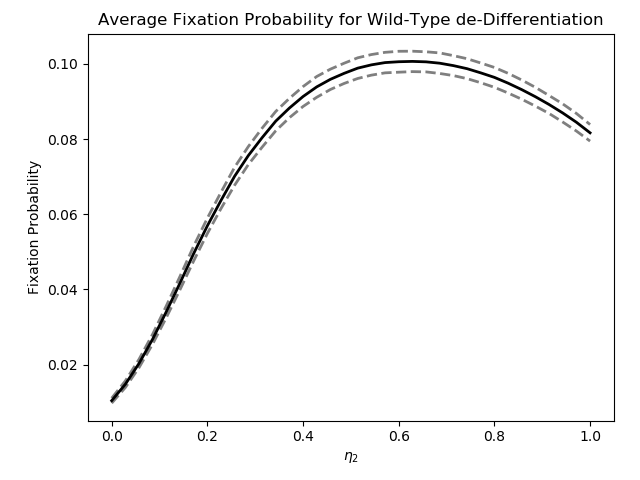
\includegraphics[width=0.74\textwidth]{avg_eta1_plot.png}
\end{center}
\caption{The mean fixation probability as a function of $\eta_2$ with the mean taken over the parameter $\eta_1$ assuming a uniform distribution. The dashed bars indicate a single deviation by standard error of the mean.}\label{avg_eta1_plot}
\end{figure}

\subsection{Stability Analysis}

The previous results were all obtained for the neutral mutant. To demonstrate the generality of these results and their independence on particular parameter choices, we repeated the analysis for varying parameters. In particular we varied the relative fitness of the mutant-types, $r_2=\tilde{r}_2$, and the probability of differentiation of the mutant types, $u_2$. The technical details can be found in Appendix \ref{exp}.


\begin{figure}[!ht]
\begin{center}
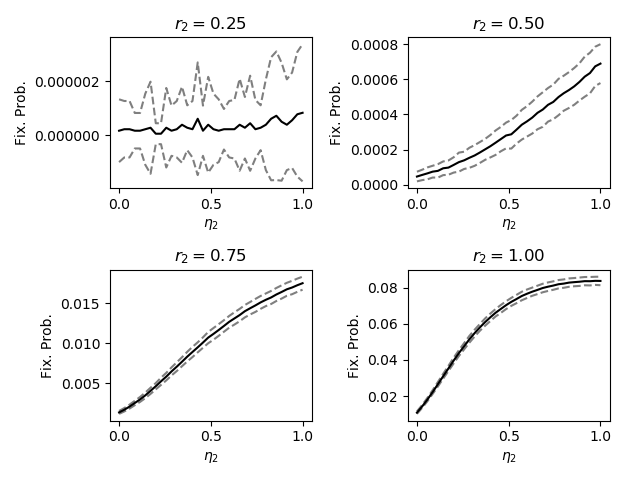
\includegraphics[width=0.74\textwidth]{avg_eta1_r2_stackplot1.png}\\
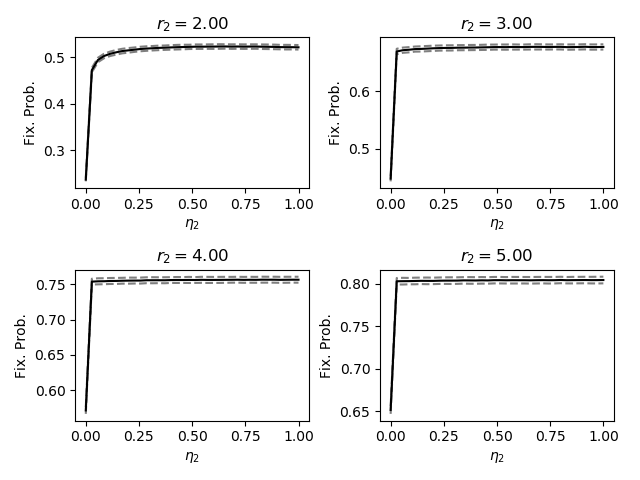
\includegraphics[width=0.74\textwidth]{avg_eta1_r2_stackplot2.png}
\end{center}
\caption{Average fixation probability for various relative fitness levels of the mutant-type cells, $r_2=\tilde{r}_2$. The dashed lines indicate one deviation of the standard error of the mean. The average was taken over wild-type de-differentiation probability $\eta_1$.}\label{r2_stack}
\end{figure}

The results of Figure \ref{r2_stack} show that for general mutant

\begin{figure}[!ht]
\begin{center}
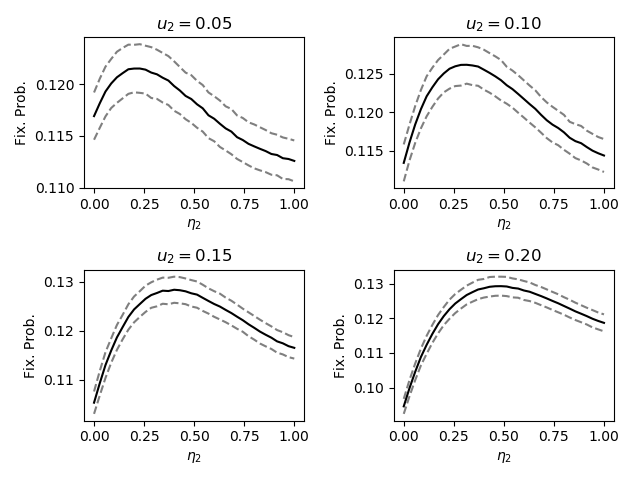
\includegraphics[width=0.74\textwidth]{avg_eta1_u2_stackplot1.png}
\end{center}
\caption{}\label{u2_stack1}
\end{figure}

\begin{figure}[!ht]
\begin{center}
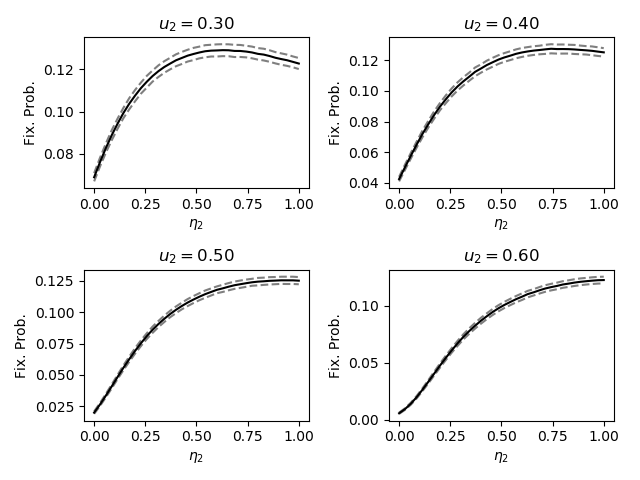
\includegraphics[width=0.74\textwidth]{avg_eta1_u2_stackplot2.png}
\end{center}
\caption{}\label{u2_stack2}
\end{figure}

\begin{figure}[!ht]
\begin{center}
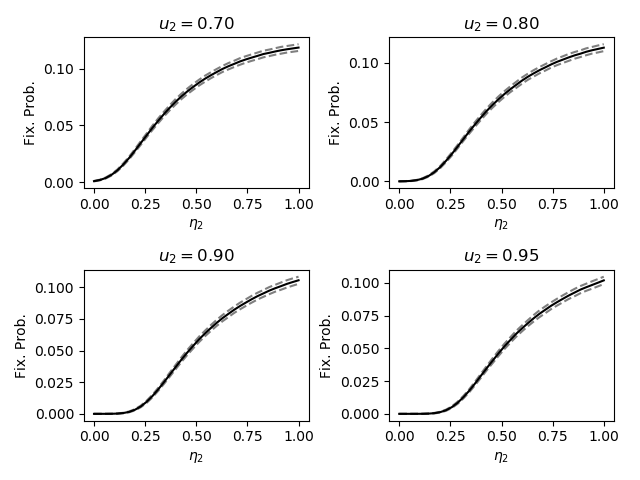
\includegraphics[width=0.74\textwidth]{avg_eta1_u2_stackplot3.png}
\end{center}
\caption{}\label{u2_stack3}
\end{figure}


\section{Conclusion}
In conclusion, two, apparently contradictory, stochastic models of cancer stem cell behaviour were considered. Both models were questioning the invasive capacity of mutant stem cells in the presence of a pre-existing stem cell and differentiated cell strata. The models were concerned with how the phenotypic plasticity, or de-differentiation rate, affected the invasive potential of these mutant stem cells. A Moran, Markovian, birth-death model was considered and Gillespie simulations of a reaction network were considered. The apparent discrepancy between these models was discovered to be hidden within assumptions determining how both the resident type and mutant type plasticity rates alter. This apparent contradiction was resolved and the behaviour of the Gillespie simulation model was recovered in the Moran context, likewise the behaviour of the Moran simulation model was recovered in the Gillespie simulation context.

ALSO I DID OTHER THINGS LIKE IN FURTHER RESULTS SECTION.

\begin{appendices}

\section{Numerics}\label{exp}

The data were generated by performing Moran simulations. Each simulation was run until fixation or extinction of the mutant stem cells occurred or until 15,000 iterations were achieved -- whichever came first. A total of 500,000 such simulations were run in 50 batches of 10,000. For each batch of 10,000 simulations, fixation probability was estimated by logging what percentage of the 10,000 iterations fixated. The error of these probabilities was estimated as the standard error of the mean calculated from the 50 different batches. 

This process was repeated for a number of $(\eta_1, \eta_2, u_2)$ sets where $\eta_1$ and $\eta_2$ vary over a discretisation of the unit square with 36 equidistant points between 0 and 1 inclusive and $u_2$ was taken from $0.05$ to $0.95$ in increments of $0.05$. The remaining parameters were given as $r_1=\tilde{r}_1=1$, $r_2=\tilde{r}_2=1.1$, $u_1=0.5$, $N_D=N_S=10$, and $d_1=d_2=\tilde{d}_1=\tilde{d}_2=1$. Each simulation began by initially considering a single mutant stem cell in a population of wild-type cells.

Similarly the procedure was repeated for a number of $(\eta_1, \eta_2, r)$ pairs where $\eta_1$ and $\eta_2$ vary as above and $r=r_2=\tilde{r}_2$ varied over the set $\{0.25, 0.5, 0.75, 1, 2, 3, 4, 5\}$. The remaining parameters were given a $r_1=\tilde{r}_1=1$, $u_2=u_1=0.5$, $N_D=N_S=10$, and$d_1=d_2=\tilde{d}_1=\tilde{d}_2=1$.

The data, and the code to generate the data, can be found at \url{https://www.github.com/brydon/StemCells2018/}

\end{appendices}

\bibliographystyle{apalike}
\bibliography{project}
\end{document}
